\documentclass[fontsize=12]{article}

\pagestyle{empty}

\usepackage{amsmath}
\usepackage{amsfonts}
\usepackage{amssymb}
\usepackage{mathtools}
\usepackage{rotating}
\usepackage{enumerate}
\usepackage[normalem]{ulem}
\usepackage{listings}
\usepackage[dvipsnames]{xcolor} %allows use of color
\usepackage{physics}
\usepackage{hyperref}
\usepackage{graphicx}
\usepackage{nicefrac}
\usepackage{cancel}
\usepackage{tcolorbox}
%\usepackage{color}
%\usepackage{listings}

\newcommand{\kB}{k_{\mathrm{B}}}
\newcommand{\kT}{\kB T}

\newcommand{\vek}[1]{\boldsymbol{#1}}          % vector symbol
\newcommand{\dif}{\mathrm{d}}                  % the d in integrals
\newcommand{\me}{\mathrm{e}}                   % Euler's e
\newcommand{\vekprod}{\! \cdot \!}
\newcommand{\eexp}[1]{\me^{\displaystyle #1}}
\newcommand{\eeexp}[1]{\me^{#1}}
\newcommand{\eeeexp}[1]{\exp \left( #1 \right)}
\newcommand{\mean}[1]{\langle#1\rangle}

\newcommand{\orderof}[1]{\mathcal{O}\left(#1\right)}
\def\Real{\hbox{I\kern-.1667em\hbox{R}}}
\newcommand{\ffrac}[2]{\frac{\displaystyle #1}{\displaystyle #2}}
\renewcommand{\Re}{\operatorname{Re}}
\renewcommand{\Im}{\operatorname{Im}}
\newcommand{\dt}{\delta t}
\newcommand{\tdt}{t + \delta t}

\newcommand{\half}{\mbox{$\frac{1}{2}$}}
\newcommand{\Phat}{\mbox{$\hat P$}}
\newcommand{\Ahat}{\mbox{$\hat A$}}
\newcommand{\ekin}{\hat{E}_{kin}} 
\newcommand{\cx}{$\cos{\xi}$}
\newcommand{\sx}{$\sin{\xi}$}
\newcommand{\csx}{$\cos^2{\xi}$}
\newcommand{\ssx}{$\sin^2{\xi}$}
\newcommand{\myx}{\ensuremath{\Delta\omega t}}
\newcommand{\hmyx}{\ensuremath{\frac{\Delta\omega t}{2}}}
\definecolor{MyGreen}{RGB}{27, 94, 20}
\newcommand*{\soln}[1]{\color{MyGreen}{{#1}}\color{black}}
\newcommand*{\solution}{\soln{Solution}}
\newcommand{\lnpar}[1]{\ln{ \left( #1 \right)}}
\newcommand{\ftexp}{\eexp{-i\va{k}\va{r}}}

\setlength{\oddsidemargin}{0.25cm}
\setlength{\textwidth}{6in}
\setlength{\topmargin}{0in}
\setlength{\headsep}{0in}
\setlength{\textheight}{8.9in}

\newcounter{problemcounter}  
\newenvironment{problemlist}
 {\begin{list}{\textbf{Problem \arabic{problemcounter}.}~}{\usecounter{problemcounter} \labelsep=0em \labelwidth=0em \leftmargin=0em \itemindent=0em}}
 {\end{list}}


\begin{document}
\begin{center}
\textbf{Homework Set 3} \\
Chemistry 553, Spring 2021 \\
Instructor: Lutz Maibaum \\
\vspace{1em}
\textbf{Due Friday, April 23th}
\end{center}

%\lstset{frame=shadowbox, rulesepcolor=\color{blue}}
%\lstinputlisting{/Users/lutz/c/python/ljmd/ljmd.py}

\begin{problemlist}

\item One the previous homework, you have shown that the Helmholtz free energy for an ideal gas in the canonical ($NVT$) ensemble is
\begin{equation*}
F(N,V,T) = - \kT \ln \ffrac{V^N}{N! \Lambda^{3N}}
\end{equation*}
where
\begin{equation*}
\Lambda = \ffrac{h}{\sqrt{2\pi m \kT}} 
\end{equation*}
is the thermal De Broglie wavelength. Here, we will explore some more properties of the ideal gas, which is an important foundation for understanding the effect of non-ideal behavior.
\begin{enumerate}[(a)~]
\item Calculate the entropy $S(N,V,T) = - \ffrac{\partial F}{\partial T}$.
\soln{
	\begin{align*}
		-\pdv{F}{T} &= -\pdv{}{T}\left[-\kT\ln{\frac{V^N}{N!\left(\frac{h}{\sqrt{2\pi m\kT}}\right)^{3N}}}\right]\\
		&= -\pdv{}{T}\left[-\kT \ln{\frac{V^N\left(2\pi m\kT\right)^{\nicefrac{3N}{2}}}{N!h^{3N}}}\right]\\
		&= -\pdv{}{T}\left[-\kT \left(\ln{\left(2\pi m\kT\right)^{\nicefrac{3N}{2}}} + \ln{\frac{V^N}{N!h^{3N}}}\right)\right]\\
		&= -\pdv{}{T}\left[-kT \left(\frac{3N}{2}\ln{T} + \ln{\frac{V^N\left(2\pi mk_B\right)^{\nicefrac{3N}{2}}}{N!h^{3N}}}\right)\right]\\
		&= -\left[-k_B\frac{3N}{2}\left(\ln{T} + 1\right) -k_B\ln{\frac{V^N\left(2\pi mk_B\right)^{\nicefrac{3N}{2}}}{N!h^{3N}}}\right]\\
		&= k_B\left(\ln{\left(Te\right)^{\nicefrac{3N}{2}}} +\ln{\frac{V^N\left(2\pi mk_B\right)^{\nicefrac{3N}{2}}}{N!h^{3N}}}\right) \\
		&= k_B\ln{\left(\frac{(Te)^{\nicefrac{3N}{2}}V^N(2\pi mk_B)^{3N/2}}{N!h^{3N}}\right)}\\
		&= k_B\ln{\left(\frac{e^{\nicefrac{3N}{2}}V^N(2\pi m\kT)^{\nicefrac{3N}{2}}}{N!h^{3N}}\right)}\\
		&= k_B\lnpar{\frac{e^{\nicefrac{3N}{2}}\ V^N}{N!\ \Lambda^{3N}}}\\
	\end{align*}
}
\item Calculate the internal energy $E(N,V,T) = F(N,V,T) + T S(N,V,T).$
\soln{
	\begin{align*}
		E(N,V,T) &= F(N,V,T) + TS(N,V,T)\\
		&= -\kT\lnpar{\frac{V^N}{N!\ \Lambda^{3N}}} + \kT\lnpar{\frac{e^{\nicefrac{3N}{2}}\ V^N}{N!\ \Lambda^{3N}}}\\
		&= \kT\lnpar{\frac{e^{\nicefrac{3N}{2}}\ V^N}{N!\ \Lambda^{3N}}\ \frac{V^N}{N!\ \Lambda^{3N}}}\\
		&= \kT\lnpar{e^{\nicefrac{3N}{2}}}\\
		&= \frac{3N}{2}\kT
	\end{align*}
}
\item In the thermodynamic limit where $N$ is large, we can use Stirling approximation, $\ln N! \approx N \ln N - N$. Use this approximation to derive a simpler expression for the Helmholtz free energy $F(N,V,T)$. Then calculate the chemical potential $\mu (N,V,T) = \ffrac{\partial F}{\partial N}$.
\soln{
	\begin{align*}
		F(N,V,T) &= -\kT\lnpar{\frac{V^N}{N!\ \Lambda^{3N}}}\\
		&= -\kT\left(\lnpar{\frac{V^N}{\Lambda^{3N}}} - \lnpar{N!}\right) \\
		&= -\kT\left(\lnpar{\frac{V^N}{\Lambda^{3N}}} - \left(N\ln{N} - N\right)\right) \\
		&= -\kT N\left(\lnpar{\frac{V}{\Lambda^{3}}} - \lnpar{\frac{N}{e}}\right) \\
		&= -kTN\lnpar{\frac{Ve}{\Lambda^3N}}\\
		\mu(N,V,T) &= \pdv{F}{N} = \pdv{}{N}\left[-kTN\lnpar{\frac{Ve}{\Lambda^3N}}\right]\\
		&= \pdv{}{N}\left[-\kT N\lnpar{\frac{Ve}{\Lambda^3}} + \kT N\lnpar{N}\right]\\
		&= -\kT\lnpar{\frac{Ve}{\Lambda^3}} + \kT\left(\ln{N} + 1\right)\\
		&= \kT\lnpar{\frac{N\Lambda^3}{V}}
	\end{align*}
}
\item Calculate the one-body density $\rho^{(1)}(\vek{r})$.
\soln{
	\begin{align*}
		\rho^{(1)}(\va{r}) &= N\omega^{(1)}(\va{r}) \\
		&= N\mean{\delta(\va{r_1}-\va{r})}\\
		&= \frac{N\int\,d\va{r_1}\,d\va{r_2}...\,d\va{r_N}\delta(\va{r_1}-\va{r})\eexp{-\beta u(\va{r_1},\va{r_2},...,\va{r_N})}}{Z} \\
		&= \frac{N\int\,d\va{r_2}...\,d\va{r_N}\eexp{-\beta u(\va{r},\va{r_2},...,\va{r_N})}}{Z} \\
		&= \frac{N\int\,d\va{r_2}...\,d\va{r_N}\eexp{0}}{Z} \\
		&= \frac{N\ V^{N-1}}{V^N} = \frac{N}{V}
	\end{align*}
	I am not sure about the step where I expanded the expectation value of the dirac delta. That was modifed from Lutz' notes where he expanded the dirac delta for the two-body density term. I evaluated the integral in the last step in the method that we used on the second problem set to get V.
}
\item Calculate the two-body density $\rho^{(2)}(\vek{r},\vek{r}')$.
\soln{
	\begin{align*}
		\rho^{(2)}(\va{r}, \va{r'}) &= N(N-1)\omega^{(2)}(\va{r}, \va{r'}) \\
		&= N(N-1)\mean{\delta(\va{r_1}-\va{r})\delta(\va{r_2}-\va{r'})}\\
		&= \frac{N(N-1)\int\,d\va{r_1}\,d\va{r_2}...\,d\va{r_N}\delta(\va{r_1}-\va{r})\delta(\va{r_2}-\va{r'})\eexp{-\beta u(\va{r_1},\va{r_2},...,\va{r_N})}}{Z} \\
		&= \frac{N(N-1)\int\,d\va{r_3}...\,d\va{r_N}\eexp{-\beta u(\va{r},\va{r'},\va{r_3},...,\va{r_N})}}{Z} \\
		&= \frac{N(N-1)\int\,d\va{r_2}...\,d\va{r_N}\eexp{0}}{Z} \\
		&= \frac{N(N-1)\ V^{N-2}}{V^N} = \frac{N(N-1)}{V^2}
	\end{align*}
}
\item Calculate the pair correlation function $g(\vek{r},\vek{r}')$. What happens in the thermodynamic limit ($N \rightarrow \infty$)?
\soln{
	\begin{align*}
		g(\va{r}, \va{r'}) &= \frac{\rho^{(2)}(\va{r}, \va{r'})}{\rho^{(1)}(\va{r})\rho^{(1)}(\va{r})}\\
		&= \frac{\frac{N(N-1)}{V^2}}{\frac{N^2}{V^2}} = \frac{V^2N(N-1)}{V^2N^2} = \frac{N-1}{N}
	\end{align*}
	In the thermodynamic limit...
	\begin{equation*}
		\lim_{N\to \infty} \frac{N-1}{N} = 1
	\end{equation*}
}
\end{enumerate}

\item Show that the pair correlation function $g(\vek{r})$ can be expressed as
\begin{equation*}
\rho g(\vek{r}) = \ffrac{1}{N} \sum_{i \neq j} \mean{\delta(\vek{r} - (\vek{r}_j - \vek{r}_i))} .
\end{equation*}
\soln{
	$g(\va{r})$ is the probability that some pari of particles is separated by $\va{r}$\\
	I am going to start by defining $\va{r} = \va{r}' - \va{r}''$ (Yes, I got this notation from Garrett and really liked it. It clears up the confusing notation that is used in this problem set)\\
	\begin{align*}
		\rho g(\va{r}) &= \rho g(\va{r}' - \va{r}'') = \frac{N(N-1)\mean{\delta(\va{r_1}-\va{r}')\delta(\va{r_2}-\va{r}'')}}{N\mean{\delta(\va{r_1}-\va{r}')}}\\
	\end{align*}
	Since we are in a homogenous system, we can redefine $\va{r}_1$ and $\va{r}_2$ as $\va{r}_j$ and $\va{r}_i$. We can also replace the $N(N-1)$ term with a sum of all pairs\\
	\begin{align*}
		= \frac{\sum_{i\neq j}\mean{\delta(\va{r_j}-\va{r}')\delta(\va{r_i}-\va{r}'')}}{N\mean{\delta(\va{r_j}-\va{r}')}}
	\end{align*}
	We can now set $\va{r}' = \va{r}_j$. If we are finding the probability that any two particles, $\va{r}_i$ and $\va{r}_j$, are separated by $\va{r}$, we can assume that  $\va{r}_j$ is at $\va{r}'$ then find the probability that any particle, $\va{r}_i$ is $\va{r}$ away.
	\begin{align*}
		&= \frac{\sum_{i\neq j}\mean{\delta(\va{r}'-\va{r}')\delta(\va{r_i}-\va{r}'')}}{N\mean{\delta(\va{r}'-\va{r}')}}\\
		&= \frac{1}{N}\sum_{i\neq j}\delta(\va{r_i}-\va{r}'')\\
		&= \frac{1}{N}\sum_{i\neq j}\delta(\va{r}-(\va{r}_j -\va{r}_i))\\
	\end{align*}
}
\item Consider a system of $N$ atoms, and an arbitrary observable $\hat{X} (\vek{r}^N)$. Let $P (x) \equiv P(\hat{X}(\vek{r}^N)=x)$ be the probability that the observable $\hat{X}$ takes on the value $x$. We have seen in class that this probability can be expressed as an expectation value of a Dirac delta function:
\begin{eqnarray*}
P (x) & =  & \mean{\delta(X(\vek{r}^N)-x)} \\
& = & \ffrac{\int \dif \vek{r}^N \, \delta(X(\vek{r}^N)-x) \, \eexp{-\beta U(\vek{r}^N)}}{\int \dif \vek{r}^N \,  \eexp{-\beta U(\vek{r}^N)}}
\end{eqnarray*}
In the last expression, the integrations are over all possible positions of all $N$ atoms, and the denominator is simply the configuration integral $Z$.
We can interpret the numerator as the configuration integral of a system in which we allow only those configurations that satisfy the constraint $X(\vek{r}^N)=x$:
\begin{equation*}
\int \limits_{\mathclap{\text{all configurations}}} \dif \vek{r}^N \, \delta(X(\vek{r}^N)-x) \, \eexp{-\beta U(\vek{r}^N)}
\approx
\int \limits_{\mathclap{\substack{\text{all configurations} \\ \text{that satisfy } X(\vek{r}^N)=x}}}  \dif \vek{r}^N \, \eexp{-\beta U(\vek{r}^N)}
\end{equation*}
Let's call this expression, the configuration integral of our system where $X$ is constrained to be equal to $x$, $Z_x$. (Note that I used an ``approximately equal'' sign -- for the purpose of this problem you can treat it as an equality.)
\begin{enumerate}[(a)~]
\item Calculate the change in free energy between the unconstrained system and the constrained system. Express this change in terms of $P(x)$.\\
\soln{
Assuming this system can be described using the canonical partition function, we can use the relationship that we proved in problem set 2, $F = F^{id} + F^{ex}$. I will use a subscript x to denote the constrained system
\begin{align*}
	F_x -F &= F_x^{id} + F_x^{ex} - F^{id} - F^{ex}\\
	&= \cancel{-\kT \lnpar{\frac{Ve}{NV^3}}} - \kT\lnpar{\frac{Z}{V^N}} + \cancel{\kT \lnpar{\frac{Ve}{NV^3}}} + \kT\lnpar{\frac{Z_x}{V^N}} \\
	&= \kT\lnpar{\frac{Z_x}{V^N}} - \kT\lnpar{\frac{Z}{V^N}}\\
	&= \kT\lnpar{\frac{Z_x}{Z}}\\
	&= -\kT\lnpar{\ffrac{\int \dif \vek{r}^N \, \delta(X(\vek{r}^N)-x) \, \eexp{-\beta U(\vek{r}^N)}}{\int \dif \vek{r}^N \,  \eexp{-\beta U(\vek{r}^N)}}}\\
	&= -\kT\lnpar{P(x)}
\end{align*}
}
\item Calculate the change in free energy when changing the constraint from on value $x_1$ to another value $x_2$. Express this change in terms of $P(x)$.
\soln{
	\begin{align*}
		-\kT\lnpar{P(x_1)} - -\kT\lnpar{P(x_2)} = -\kT\lnpar{\frac{P(x_1)}{P(x_2)}}
	\end{align*}
}
\end{enumerate}

\item In this problem you are asked to show some very useful properties of Fourier transforms. The Fourier transform of a function $f(\vek{r})$ is
\begin{equation*}
\tilde{f}(\vek{k})  =  \int \eexp{- i \vek{k}\vekprod\vek{r}} f(\vek{r}) \, \dif\vek{r} 
\end{equation*}
and you can go back to your original function by the inverse Fourier transform,
\begin{equation*}
f(\vek{r})  =  \frac{1}{\left(2 \pi\right)^d} \int \eexp{i \vek{k}\vekprod\vek{r}} \tilde{f}(\vek{k}) \, \dif\vek{k} .
\end{equation*}
Here $d$ is the dimensionality of the system, usually $d=3$ for our applications.

\begin{enumerate}[(a)~]
\item Calculate the Fourier transform of the Dirac $\delta$ function, $f(\vek{r}) = \delta(\vek{r}-\vek{r}')$.
\soln{
	\begin{align*}
		\tilde{f}(\va{k}) &= \int \eexp{-i\va{k}\va{r}}f(\va{r})\\
		&= \int\eexp{-i\va{k}\va{r}}\delta(\va{r} - \va{r}')\\
		&= \eexp{-i\va{k}\va{r}'}
	\end{align*}
}
\item Show that
\begin{equation*}
\delta(\vek{r}-\vek{r}') = \frac{1}{\left(2 \pi\right)^d} \int \eexp{i \vek{k} \vekprod (\vek{r}-\vek{r}')} \, \dif \vek{k}
\end{equation*}
\soln{
	\begin{align*}
		f(\va{r}) &= \delta(\va{r} - \va{r'}) = \frac{1}{(2\pi)^d}\int \eexp{-i\va{k}\va{r}}\tilde{f}(\va{k})\,d{\va{k}}\\
		&= \frac{1}{(2\pi)^d}\int \eexp{-i\va{k}\va{r}}\eexp{-i\va{k}\va{r'}}\,d{\va{k}}\\
		&= \frac{1}{(2\pi)^d}\int \eexp{-i\va{k}\left(\va{r}-\va{r'}\right)}\,d{\va{k}}\\
	\end{align*}
}
\item Show that if the function $f$ is the gradient of another function $\phi$,
\begin{equation*}
f(\vek{r}) = \vek{\nabla} \phi(\vek{r}) ,
\end{equation*}
then its Fourier transform is
\begin{equation*}
\tilde{f}(\vek{k}) = i \vek{k} \tilde{\phi}(\vek{k}) .
\end{equation*}
(Note: if you do an integration by parts, you can ignore the boundary term at infinity). This is a very useful property of the Fourier transform: it turns the derivative operator into a simple multiplication with $i \vek{k}$.
\soln{
	\begin{align*}
		\tilde{f}(\va{k}) &= \int \eexp{-i\va{k}\va{r}}\nabla\phi(\va{r})\,dr\\
	\end{align*}
	\begin{tcolorbox}[title=Integration by Parts]
	\begin{align*}
		u &= \eexp{-i\va{k}\va{r}}\\
		du &= -i\va{k}\eexp{-i\va{k}\va{r}} d\va{r}\\
		dv &= \nabla\phi(\va{r})\,dr \\
		v &= \phi(\va{r})
	\end{align*}
	\end{tcolorbox}
	\begin{align*}
		\int u\,dv &= uv-\int v\,du\\
		&= \eexp{-i\va{k}\va{r}}\phi(\va{r}) - \int \phi(\va{r})\left(-i\va{k}\eexp{-i\va{k}\va{r}}\right) d\va{r}\\
		&= \eexp{-i\va{k}\va{r}}\phi(\va{r}) + i\va{k}\int \phi(\va{r})\eexp{-i\va{k}\va{r}} d\va{r}\\
		&= \cancel{\eexp{-i\va{k}\va{r}}\phi(\va{r})} + i\va{k}\tilde{\phi}(\va{k})
	\end{align*}
	And for some reason, the first term fucks off
}
\item Show that if the function $f$ is a \emph{convolution} of two other functions $g$ and $h$,
\begin{equation*}
 f(\vek{r})  =  \int \dif \vek{r}' \, g(\vek{r}') h (\vek{r}-\vek{r}')  ,
\end{equation*}
then its Fourier transform is
\begin{equation*}
\tilde{f}(\vek{k}) =  \tilde{g}(\vek{k}) \tilde{h}(\vek{k}) .
\end{equation*}
\soln{
	\begin{align*}
		\tilde{f}(\va{r}) &= \int \ftexp f(\va{r})\,d{\va{r}} \\
		&= \int \ftexp \int \,d{\va{r'}}g(\va{r'})h(\va{r}-\va{r'})\,d{\va{r}} \\
		&= \int \int \ftexp g(\va{r'})h(\va{r}-\va{r'})\,d{\va{r'}}\,d{\va{r}}\\
		& \text{Now we let $u = \va{r}-\va{r'}$} \\
		&= \int \int \eexp{-i\va{k}(\va{u} + \va{r'})} g(\va{r'})h(\va{u})\,d{\va{r'}}\,d{\va{u}}\\
		&= \text{ I am saying that $d\va{r} = d\va{u}$ but I cant really show why} \\
		&= \int \int \eexp{-i\va{k}\va{u}}\eexp{-i\va{k}\va{r'}} g(\va{r'})h(\va{u})\,d{\va{r'}}\,d{\va{u}}\\
		&= \int\eexp{-i\va{k}\va{u}}h(\va{u})\,d{\va{u}}\int \eexp{-i\va{k}\va{r'}}g(\va{r'})\,d{\va{r'}} \\
		&= \tilde{g}(\va{k})\tilde{h}(\va{k})
	\end{align*}
}
\item Consider the case where $d=3$. Show that if the function $f$ is isotropic,
\begin{equation*}
 f(\vek{r})  =  f(r) ,
\end{equation*}
then so is its Fourier transform $\tilde{f}(\vek{k})$, and the latter can be computed as
\begin{equation*}
\tilde{f}(k) = 4 \pi \int_0^\infty r^2 f(r) \frac{\sin (kr)}{kr} \, \dif r .
\end{equation*}
\soln{
	\begin{align*}
		\tilde{f}(\va{k})  &= \int \ftexp f(\va{r})\,d{\va{r}} \\
		&= \int_0^{2\pi}\int_0^\pi\int_0^\infty f(r) \eexp{-ikr\cos{\theta}}r^2\,dr \sin{\theta}\,d\theta\,d\phi \\
		& \text{ now we do u-sub with $u = -\cos{\theta}$ and $du = \sin{\theta}d\theta$}\\
		&= 2\pi \int_{-1}^1\int_0^\infty f(r)\eexp{-ikru}r^2\,dr\,du\\
		&= 2\pi \int_0^\infty \left[\frac{1}{ikr}\eexp{ikru}\right]_{-1}^1f(r)r^2\,dr\\
		&=2\pi \int_0^\infty \left[\frac{-\eexp{ikr}}{ikr}-\frac{-\eexp{-ikr}}{ikr}\right]f(r)r^2\,dr\\
		&= 2\pi \int_0^\infty \frac{1}{ikr}\left(\cos{kr} + i\sin{kr} -\cos{kr} + i\sin{kr}\right)f(r)r^2\,dr\\
		&= 2\pi \int_0^\infty \frac{1}{kr}\left(2\sin{kr}\right)f(r)r^2\,dr\\
		&= 4\pi \int_0^\infty r^2f(r)\frac{\sin{kr}}{kr}\,dr\\
	\end{align*}
}\\
Note that the converse is also true (you don't have to show this, because it's the exact same calculation as before): if $\tilde{f}$ is isotropic ($\tilde{f}(\vek{k}) = \tilde{f}(k)$), then so is the inverse Fourier transform $f$, which is then given by
\begin{equation*}
f(r) = \ffrac{1}{2\pi^2} \int_0^\infty \dif k \, k^2 \tilde{f}(k) \ffrac{\sin (kr)}{kr} .
\end{equation*}
\end{enumerate}

\item Work through the attached notebook "Molecular Dynamics II - Atomic Collisions". It contains 4 exercises that you should do and turn in.
\soln{
\begin{enumerate}
	\item The two plots shown below are the x-coordinates and the energy for two particles interacting with a Weeks-Chandler-Anderson (WCA) potential.\\
	\item 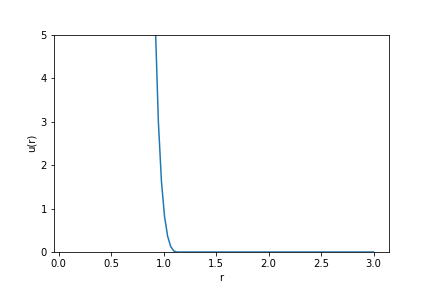
\includegraphics[scale=0.5]{wca_pot}\\
	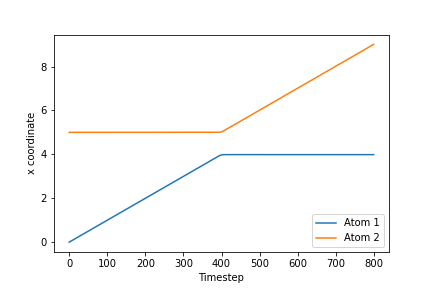
\includegraphics[scale=0.5]{two_spheres_x}
	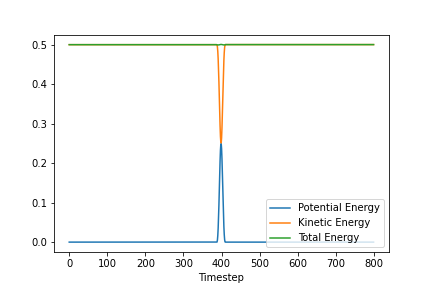
\includegraphics[scale=0.5]{two_spheres_e}
	The x-position plot shows atom 1 moving toward atom 2 until they reach some distance where they start interacting. The WCA potential only has repulsive interactions so as soon as the atoms interact, the kinetic energy of atom 1 is transferred to atom 2.
	\item The next two plots are the same x-coordinate and energy plots as in exercise 1, but were generated using the Lennard-Jones (LJ) potential instead of the WCA potential\\
	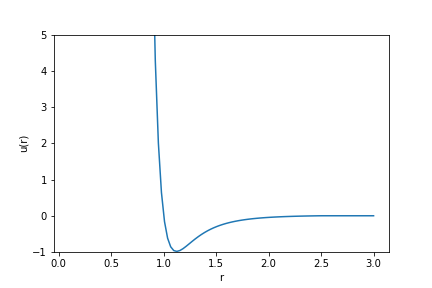
\includegraphics[scale=0.5]{LJ_pot}\\
	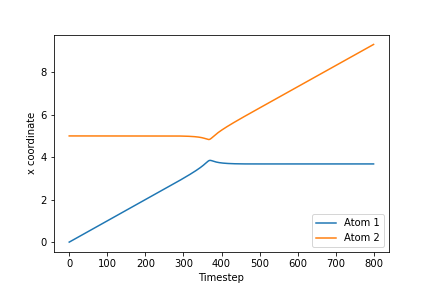
\includegraphics[scale=0.5]{LJ_two_x}
	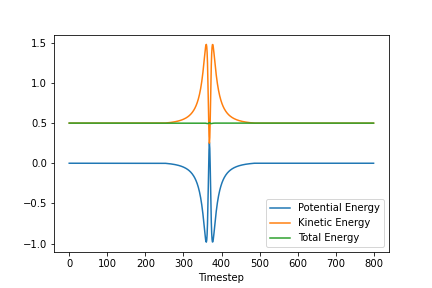
\includegraphics[scale=0.5]{LJ_two_e}
	The difference between these plots and the plots above is due to the difference in the potentials used. The LJ potential contains attractive interactions when the particles are close to each other. As atom 1 gets close to atom 2, both experience an attractive force equal in magnitude, but opposite in direction causing the kinetic energy of both particles to increase. Once they reach a certain distance, the attractive force become repulsive and the atoms begin to move apart. 
	\item When the one atom hits the cluster of atoms, the kinetic energy is transferred from atom to atom, but none of the atoms gain enough kinetic energy to escape the potential well so they stay in a cluster
	\item When the initial velocity of atom 1 is increase, it hits the cluster with more kinetic energy. That kinetic energy is transferred to the other atoms, giving two of them enough energy to escape the potential well and move out of the cluster. 
\end{enumerate}
}

\end{problemlist}  % enumeration of problems

%\begin{enumerate}[(a)~]
%\item
%\end{enumerate}

\end{document}
